\documentclass{ximera}

 

\usepackage{epsfig}

\graphicspath{
  {./}
  {figures/}
}

\usepackage{morewrites}
\makeatletter
\newcommand\subfile[1]{%
\renewcommand{\input}[1]{}%
\begingroup\skip@preamble\otherinput{#1}\endgroup\par\vspace{\topsep}
\let\input\otherinput}
\makeatother

\newcommand{\includeexercises}{\directlua{dofile("/home/jim/linearAlgebra/laode/exercises.lua")}}

%\newcounter{ccounter}
%\setcounter{ccounter}{1}
%\newcommand{\Chapter}[1]{\setcounter{chapter}{\arabic{ccounter}}\chapter{#1}\addtocounter{ccounter}{1}}

%\newcommand{\section}[1]{\section{#1}\setcounter{thm}{0}\setcounter{equation}{0}}

%\renewcommand{\theequation}{\arabic{chapter}.\arabic{section}.\arabic{equation}}
%\renewcommand{\thefigure}{\arabic{chapter}.\arabic{figure}}
%\renewcommand{\thetable}{\arabic{chapter}.\arabic{table}}

%\newcommand{\Sec}[2]{\section{#1}\markright{\arabic{ccounter}.\arabic{section}.#2}\setcounter{equation}{0}\setcounter{thm}{0}\setcounter{figure}{0}}

\newcommand{\Sec}[2]{\section{#1}}

\setcounter{secnumdepth}{2}
%\setcounter{secnumdepth}{1} 

%\newcounter{THM}
%\renewcommand{\theTHM}{\arabic{chapter}.\arabic{section}}

\newcommand{\trademark}{{R\!\!\!\!\!\bigcirc}}
%\newtheorem{exercise}{}

\newcommand{\dfield}{{\sf dfield9}}
\newcommand{\pplane}{{\sf pplane9}}

\newcommand{\EXER}{\section*{Exercises}}%\vspace*{0.2in}\hrule\small\setcounter{exercise}{0}}
\newcommand{\CEXER}{}%\vspace{0.08in}\begin{center}Computer Exercises\end{center}}
\newcommand{\TEXER}{} %\vspace{0.08in}\begin{center}Hand Exercises\end{center}}
\newcommand{\AEXER}{} %\vspace{0.08in}\begin{center}Hand Exercises\end{center}}

% BADBAD: \newcommand{\Bbb}{\bf}

\newcommand{\R}{\mbox{$\Bbb{R}$}}
\newcommand{\C}{\mbox{$\Bbb{C}$}}
\newcommand{\Z}{\mbox{$\Bbb{Z}$}}
\newcommand{\N}{\mbox{$\Bbb{N}$}}
\newcommand{\D}{\mbox{{\bf D}}}
\usepackage{amssymb}
%\newcommand{\qed}{\hfill\mbox{\raggedright$\square$} \vspace{1ex}}
%\newcommand{\proof}{\noindent {\bf Proof:} \hspace{0.1in}}

\newcommand{\setmin}{\;\mbox{--}\;}
\newcommand{\Matlab}{{M\small{AT\-LAB}} }
\newcommand{\Matlabp}{{M\small{AT\-LAB}}}
\newcommand{\computer}{\Matlab Instructions}
\newcommand{\half}{\mbox{$\frac{1}{2}$}}
\newcommand{\compose}{\raisebox{.15ex}{\mbox{{\scriptsize$\circ$}}}}
\newcommand{\AND}{\quad\mbox{and}\quad}
\newcommand{\vect}[2]{\left(\begin{array}{c} #1_1 \\ \vdots \\
 #1_{#2}\end{array}\right)}
\newcommand{\mattwo}[4]{\left(\begin{array}{rr} #1 & #2\\ #3
&#4\end{array}\right)}
\newcommand{\mattwoc}[4]{\left(\begin{array}{cc} #1 & #2\\ #3
&#4\end{array}\right)}
\newcommand{\vectwo}[2]{\left(\begin{array}{r} #1 \\ #2\end{array}\right)}
\newcommand{\vectwoc}[2]{\left(\begin{array}{c} #1 \\ #2\end{array}\right)}

\newcommand{\ignore}[1]{}


\newcommand{\inv}{^{-1}}
\newcommand{\CC}{{\cal C}}
\newcommand{\CCone}{\CC^1}
\newcommand{\Span}{{\rm span}}
\newcommand{\rank}{{\rm rank}}
\newcommand{\trace}{{\rm tr}}
\newcommand{\RE}{{\rm Re}}
\newcommand{\IM}{{\rm Im}}
\newcommand{\nulls}{{\rm null\;space}}

\newcommand{\dps}{\displaystyle}
\newcommand{\arraystart}{\renewcommand{\arraystretch}{1.8}}
\newcommand{\arrayfinish}{\renewcommand{\arraystretch}{1.2}}
\newcommand{\Start}[1]{\vspace{0.08in}\noindent {\bf Section~\ref{#1}}}
\newcommand{\exer}[1]{\noindent {\bf \ref{#1}}}
\newcommand{\ans}{}
\newcommand{\matthree}[9]{\left(\begin{array}{rrr} #1 & #2 & #3 \\ #4 & #5 & #6
\\ #7 & #8 & #9\end{array}\right)}
\newcommand{\cvectwo}[2]{\left(\begin{array}{c} #1 \\ #2\end{array}\right)}
\newcommand{\cmatthree}[9]{\left(\begin{array}{ccc} #1 & #2 & #3 \\ #4 & #5 &
#6 \\ #7 & #8 & #9\end{array}\right)}
\newcommand{\vecthree}[3]{\left(\begin{array}{r} #1 \\ #2 \\
#3\end{array}\right)}
\newcommand{\cvecthree}[3]{\left(\begin{array}{c} #1 \\ #2 \\
#3\end{array}\right)}
\newcommand{\cmattwo}[4]{\left(\begin{array}{cc} #1 & #2\\ #3
&#4\end{array}\right)}

\newcommand{\Matrix}[1]{\ensuremath{\left(\begin{array}{rrrrrrrrrrrrrrrrrr} #1 \end{array}\right)}}

\newcommand{\Matrixc}[1]{\ensuremath{\left(\begin{array}{cccccccccccc} #1 \end{array}\right)}}



\renewcommand{\labelenumi}{\theenumi)}
\newenvironment{enumeratea}%
{\begingroup
 \renewcommand{\theenumi}{\alph{enumi}}
 \renewcommand{\labelenumi}{(\theenumi)}
 \begin{enumerate}}
 {\end{enumerate}\endgroup}



\newcounter{help}
\renewcommand{\thehelp}{\thesection.\arabic{equation}}

%\newenvironment{equation*}%
%{\renewcommand\endequation{\eqno (\theequation)* $$}%
%   \begin{equation}}%
%   {\end{equation}\renewcommand\endequation{\eqno \@eqnnum
%$$\global\@ignoretrue}}

%\input{psfig.tex}

\author{Martin Golubitsky and Michael Dellnitz}

%\newenvironment{matlabEquation}%
%{\renewcommand\endequation{\eqno (\theequation*) $$}%
%   \begin{equation}}%
%   {\end{equation}\renewcommand\endequation{\eqno \@eqnnum
% $$\global\@ignoretrue}}

\newcommand{\soln}{\textbf{Solution:} }
\newcommand{\exercap}[1]{\centerline{Figure~\ref{#1}}}
\newcommand{\exercaptwo}[1]{\centerline{Figure~\ref{#1}a\hspace{2.1in}
Figure~\ref{#1}b}}
\newcommand{\exercapthree}[1]{\centerline{Figure~\ref{#1}a\hspace{1.2in}
Figure~\ref{#1}b\hspace{1.2in}Figure~\ref{#1}c}}
\newcommand{\para}{\hspace{0.4in}}

\renewenvironment{solution}{\suppress}{\endsuppress}

\ifxake
\newenvironment{matlabEquation}{\begin{equation}}{\end{equation}}
\else
\newenvironment{matlabEquation}%
{\let\oldtheequation\theequation\renewcommand{\theequation}{\oldtheequation*}\begin{equation}}%
  {\end{equation}\let\theequation\oldtheequation}
\fi

\makeatother


\title{Least Squares Approximations}

\begin{document}
\begin{abstract}
\end{abstract}
\maketitle

  \label{S:LSA}

Let $W\subset\R^n$ be a subspace and $x_0\in\R^n$ be a vector.  In this
section we solve a basic geometric problem and investigate some of its
consequences.  The problem is:
\begin{quote}
Find a vector $w_0\in W$ that is the nearest vector in $W$ to $x_0$.
\end{quote}

\begin{figure}[htb]
        \centerline{%
        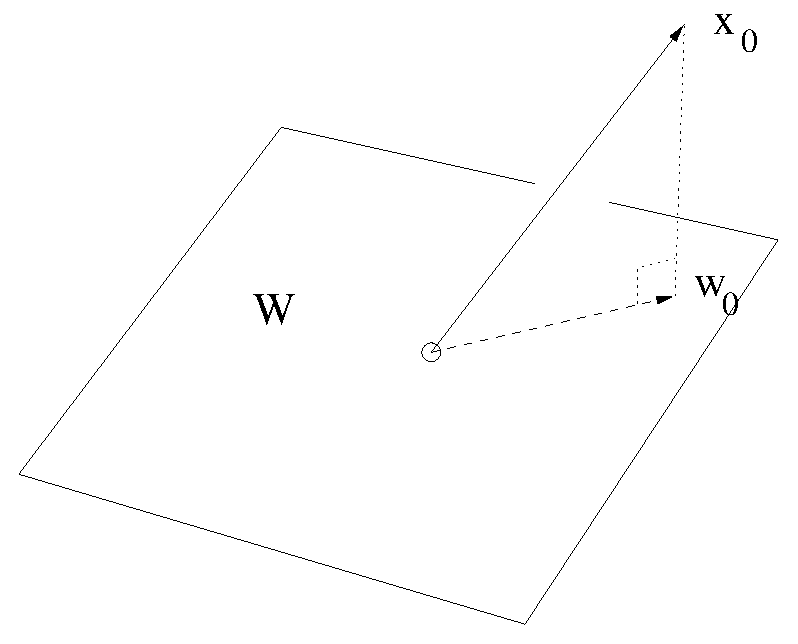
\psfig{file=../figures/nearest.eps,width=2.5in}}
        \caption{Approximation of $x_0$ by $w_0\in W$ by least squares.}
        \label{F:nearest}
\end{figure}


The distance between two vectors\index{distance!between vectors}
$v$ and $w$ is $||v-w||$ and the geometric
problem can be rephrased as follows: find a vector $w_0\in W$ such that
\begin{equation}  \label{E:leastsq}
||x_0-w_0||\leq ||x_0-w|| \quad \forall w\in W.
\end{equation}
Condition \Ref{E:leastsq} is called the
{\em least squares approximation}\index{least squares!approximation}.
In order to see where this name comes from we write\Ref{E:leastsq} in the
equivalent form
\[
||x_0-w_0||^2\leq ||x_0-w||^2 \quad \forall w\in W.
\]
This form means that for $w=w_0$ the sum of the squares of the
components of the vector $x_0-w$ is minimal.

Before continuing, we state and prove the {\em Law of Phythagorus\/}.
\index{Law of Phythagorus}  Let $z_1,z_2\in\R^n$ be orthogonal vectors.  Then 
\begin{equation} \label{E:LP}
||z_1+z_2||^2 = ||z_1||^2 + ||z_2||^2.
\end{equation}
To verify \Ref{E:LP} calculate 
\begin{align*}
  ||z_1+z_2||^2&=(z_1+z_2)\cdot(z_1+z_2) \\
  &=z_1\cdot z_1 +2z_1\cdot z_2+z_2\cdot z_2 \\
  &=||z_1||^2 + 2z_1\cdot z_2 +||z_2||^2.
\end{align*}
Since $z_1$ and $z_2$ are orthogonal, $z_1\cdot z_2=0$ and the Law of 
Phythagorus is valid.

Using \Ref{E:leastsq} and \Ref{E:LP}, we can rephrase the minimum distance 
problem as follows.
\begin{lemma}  \label{L:orthoLSA}
The vector $w_0\in W$ is the closest vector to $x_0\in\R^n$ if the vector 
$x_0-w_0$ is orthogonal to every vector in $W$. (See Figure~\ref{F:nearest}.)
\end{lemma}

\begin{proof}  Write $x_0-w=z_1+z_2$ where $z_1=x_0-w_0$ and $z_2=w_0-w$.  By 
assumption, $x_0-w_0$ is orthogonal to every vector in $W$; so $z_1$ and 
$z_2\in W$ are orthogonal.  It follows from \Ref{E:LP} that
\[
||x_0-w||^2 = ||x_0-w_0||^2 + ||w_0-w||^2.
\]
Since $||w_0-w||^2\ge 0$, \Ref{E:leastsq} is valid, and $w_0$ is the vector 
nearest to $x_0$ in $W$. \end{proof}

\subsubsection*{Least Squares Distance to a Line}
\index{least squares!distance to a line}
\index{distance!to a line}

Suppose $W$ is as simple a subspace as possible; that is, suppose $W$ is one
dimensional with basis vector $w$.  Since $W$ is one dimensional, a vector
$w_0\in W$ that is closest to $x_0$ must be a multiple of $w$; that is,
$w_0=aw$.  Suppose that we can find a scalar $a$ so that $x_0-aw$ is
orthogonal to every vector in $W$.  Then it follows from
Lemma~\ref{L:orthoLSA} that $w_0$ is the closest vector in $W$ to $x_0$.
To find $a$, calculate
\[
0 = (x_0-aw)\cdot w = x_0\cdot w - a w\cdot w.
\]
Then
\[
a = \frac{x_0\cdot w}{||w||^2}
\]
and
\begin{equation}  \label{E:singleortho}
w_0 = \frac{x_0\cdot w}{||w||^2} w.
\end{equation}
Observe that $||w||^2\not=0$ since $w$ is a basis vector.

For example, if $x_0=(1,2,-1,3)\in\R^4$ and $w=(0,1,2,3)$.  The the vector
$w_0$ in the space spanned by $w$ that is nearest to $x_0$ is
\[
w_0 = \frac{9}{14}w
\]
since $x_0\cdot w=9$ and $||w||^2=14$.

\subsubsection*{Least Squares Distance to a Subspace}
\index{least squares!distance to a subspace}
\index{distance!to a subspace}

Similarly, using Lemma~\ref{L:orthoLSA} we can solve the general least
squares problem by solving a system of linear equations.  Let
$w_1,\ldots,w_k$ be a basis for $W$ and suppose that
\[
w_0 = \alpha_1w_1 + \cdots + \alpha_kw_k
\]
for some scalars $\alpha_i$.  We now show how to find these scalars.

\begin{theorem}  \label{T:nearestvector}
Let $x_0\in\R^n$ be a vector, and let $\{w_1,\ldots,w_k\}$ be a
basis\index{basis} for the subspace\index{subspace} $W\subset\R^n$.
Then
\[
w_0 = \alpha_1w_1 + \cdots + \alpha_kw_k
\]
is the nearest vector in $W$ to $x_0$ when
\begin{equation}  \label{E:nearestvector}
\left(\begin{array}{c} \alpha_1 \\ \vdots \\ \alpha_k \end{array}\right) =
(A^tA)\inv A^tx_0,
\end{equation}
where $A=(w_1|\cdots|w_k)$ is the $n\times k$ matrix whose columns are the
basis vectors of $W$.
\end{theorem}

\begin{proof} Observe that the vector $x_0-w_0$ is orthogonal to every vector in $W$
precisely when $x_0-w_0$ is orthogonal to each basis vector $w_j$.  It
follows from Lemma~\ref{L:orthoLSA} that $w_0$ is the closest vector to $x_0$
in $W$ if
\[
(x_0-w_0)\cdot w_j = 0
\]
for every $j$.  That is, if
\[
w_0\cdot w_j = x_0\cdot w_j
\]
for every $j$.  These equations can be rewritten as a system of equations in
terms of the $\alpha_i$, as follows:
\begin{equation}  \label{E:dots}
 \begin{array}{ccc}
w_1\cdot w_1\alpha_1 + \cdots + w_1\cdot w_k\alpha_k & = & w_1\cdot x_0\\
 & \vdots &  \\
w_k\cdot w_1\alpha_1 + \cdots + w_k\cdot w_k\alpha_k & = & w_k\cdot x_0.
\end{array}
\end{equation}

Note that if $u,v\in\R^n$ are column vectors, then $u\cdot v= u^tv$. Therefore,
we can rewrite \Ref{E:dots} as
\[
A^tA \left(\begin{array}{c} \alpha_1\\ \vdots \\ \alpha_k \end{array}\right) =
A^tx_0,
\]
where $A$ is the matrix whose columns are the $w_j$ and $x_0$ is viewed as a
column vector.  Note that the matrix $A^tA$ is a $k\times k$ matrix.

We claim that $A^tA$ is invertible.  To verify this claim, it suffices to
show that the null space\index{null space}
of $A^tA$ is zero; that is, if $A^tA z = 0$ for some
$z\in\R^k$, then $z=0$.  First, calculate
\[
||Az||^2 = Az\cdot Az = (Az)^tAz = z^tA^tAz= z^t0 = 0.
\]
It follows that $Az=0$.  Now if we let $z=(z_1,\ldots,z_k)^t$, then the
equation $Az=0$ may be rewritten as
\[
z_1w_1 + \cdots + z_kw_k = 0.
\]
Since the $w_j$ are linearly independent, it follows that the $z_j=0$.  In
particular, $z=0$.  Since $A^tA$ is invertible, \Ref{E:nearestvector} is
valid, and the theorem is proved. \end{proof}


\subsection*{Gram-Schmidt Orthonormalization Process}
\index{Gram-Schmidt orthonormalization}

Suppose that ${\cal W} = \{w_1,\ldots,w_k\}$ is a basis for the subspace
$V\subset\R^n$.  There is a natural process by which the ${\cal W}$ basis
can be transformed into an
orthonormal basis\index{basis!orthonormal}
${\cal V}$ of $V$.  This
process proceeds inductively on the $w_j$; the orthonormal vectors
$v_1,\ldots,v_k$ can be chosen so that
\[
\Span\{v_1,\ldots,v_j\} = \Span\{w_1,\ldots,w_j\}
\]
\index{span}
for each $j\leq k$.  Moreover, the $v_j$ are chosen using the theory of
least squares that we have just discussed.

\subsubsection*{The Case $j=2$}

To gain a feeling for how the induction process works, we verify the case
$j=2$.  Set
\begin{equation}  \label{E:ortho1}
v_1 = \frac{1}{||w_1||}w_1;
\end{equation}
so $v_1$ points in the same direction as $w_1$ and has unit length, that is,
$v_1\cdot v_1=1$.  The normalization is shown in Figure~\ref{F:gram}.

\begin{figure}[htb]
        \centerline{%
        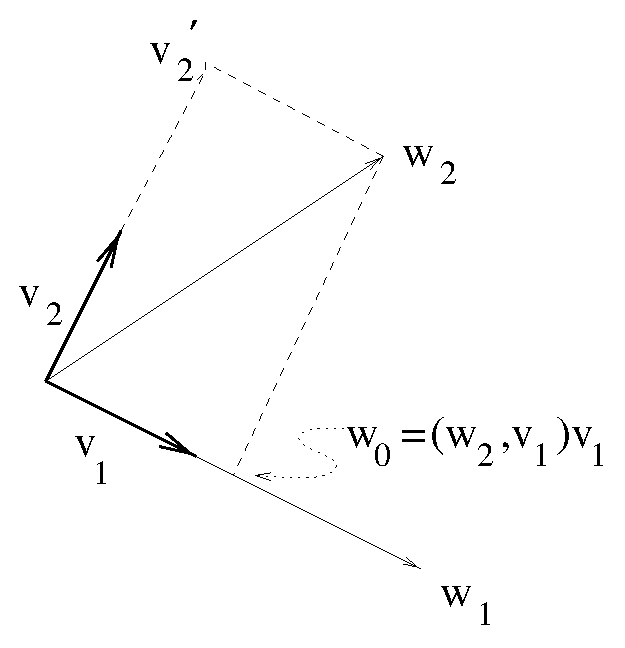
\psfig{file=../figures/gram.eps,width=2.0in}}
        \caption{Planar illustration of Gram-Schmidt orthonormalization.}
        \label{F:gram}
\end{figure}

Next, we find a unit length vector $v'_2$ in the plane spanned by $w_1$ and
$w_2$ that is perpendicular\index{perpendicular}
to $v_1$. Let $w_0$ be the vector on the line
generated by $v_1$ that is nearest to $w_2$.  It follows from
\Ref{E:singleortho} that
\[
w_0 = \frac{w_2\cdot v_1}{||v_1||^2}v_1 = (w_2\cdot v_1) v_1.
\]
The vector $w_0$ is shown on Figure~\ref{F:gram} and, as
Lemma~\ref{L:orthoLSA} states, the vector $v_2'=w_2-w_0$ is perpendicular to
$v_1$. That is,
\begin{equation}  \label{E:ortho2}
v'_2 = w_2 - (w_2\cdot v_1) v_1
\end{equation}
is orthogonal\index{orthogonal} to $v_1$.

Finally, set
\begin{equation}  \label{E:ortho3}
v_2 = \frac{1}{||v'_2||}v'_2
\end{equation}
so that $v_2$ has unit length.  Since $v_2$ and $v'_2$ point in the
same direction, $v_1$ and $v_2$ are orthogonal.  Note also that $v_1$ and
$v_2$ are linear combinations of $w_1$ and $w_2$.  Since $v_1$ and $v_2$ are
orthogonal, they are linearly independent.  It follows that
\[
\Span\{v_1,v_2\} = \Span\{w_1,w_2\}.
\]

In summary: computing $v_1$ and $v_2$ using \Ref{E:ortho1}, \Ref{E:ortho2}
and \Ref{E:ortho3} yields an orthonormal basis for the
plane\index{plane} spanned by $w_1$ and $w_2$.

\subsubsection*{The General Case}

\begin{theorem} (Gram-Schmidt Orthonormalization) \label{T:orthobasis}
Let $w_1,\ldots,w_k$ be a basis for the subspace $W\subset\R^n$.  Define
$v_1$ as in \Ref{E:ortho1} and then define inductively
\begin{align}
  v'_{j+1} & =  w_{j+1} -(w_{j+1}\cdot v_1)v_1- \cdots \nonumber\\
  &\quad -(w_{j+1}\cdot v_j)v_j \label{E:inductiveGS} \\
v_{j+1} & =  \frac{1}{||v'_{j+1}||}v'_{j+1}. \label{eq:gsnormal}
\end{align}
Then $v_1,\ldots,v_k$ is an orthonormal basis of $W$ such that for each $j$
\[
\Span\{v_1,\ldots,v_j\} = \Span\{w_1,\ldots,w_j\}
\]
\end{theorem}\index{Gram-Schmidt orthonormalization}
\index{basis!orthonormal}

\begin{proof}  We assume that we have constructed orthonormal vectors $v_1,\ldots,v_j$
such that
\[
\Span\{v_1,\ldots,v_j\} = \Span\{w_1,\ldots,w_j\}.
\]
Our purpose is to find a unit vector $v_{j+1}$ that is orthogonal to each $v_i$
and that satisfies
\[
\Span\{v_1,\ldots,v_{j+1}\} = \Span\{w_1,\ldots,w_{j+1}\}.
\]
We construct $v_{j+1}$ in two steps.  First we find a vector $v'_{j+1}$
that is orthogonal to each of the $v_i$ using least squares.  Let $w_0$
be the vector in $\Span\{v_1,\ldots,v_j\}$ that is nearest to $w_{j+1}$.
Theorem~\ref{T:nearestvector} tells us how to make this construction.
Let $A$ be the matrix whose columns are $v_1,\ldots,v_j$.  Then
\Ref{E:nearestvector} states that the coordinates of $w_0$ in the $v_i$ basis
is given by $(A^tA)\inv A^tw_{j+1}$. But since the $v_i$'s are orthonormal,
the matrix $A^tA$ is just $I_k$.  Hence
\[
w_0 =  (w_{j+1}\cdot v_1)v_1 + \cdots + (w_{j+1}\cdot v_j)v_j.
\]
Note that $v'_{j+1}=w_{j+1}-w_0$ is the vector defined in \Ref{E:inductiveGS}.
We claim that $v'_{j+1}=w_{j+1}-w_0$ is orthogonal to $v_k$ for $k\leq j$
and hence to every vector in $\Span\{v_1,\ldots,v_j\}$.  Just calculate
\[
v_{j+1}'\cdot v_k = w_{j+1}\cdot v_k - w_0\cdot v_k =
w_{j+1}\cdot v_k -  w_{j+1}\cdot v_k = 0.
\]
Define $v_{j+1}$ as in
\Ref{eq:gsnormal}.  It follows that $v_1,\ldots,v_{j+1}$ are orthonormal and
that each vector is a linear combination of $w_1,\ldots,w_{j+1}$.  \end{proof}


\subsubsection*{An Example of Orthonormalization}

Let $W\subset\R^4$ be the subspace spanned by the vectors
\begin{equation}  \label{eq:gsexam}
w_1=(1,0,-1,0),\quad w_2=(2,-1,0,1),\quad w_3=(0,0,-2,1).
\end{equation}
We find an orthonormal basis for $W$ using Gram-Schmidt orthonormalization.

\begin{description}
\item[Step 1:]   Set
\[
v_1 = \frac{1}{||w_1||}w_1=\frac{1}{\sqrt{2}}(1,0,-1,0).
\]
\item[Step 2:] Following the Gram-Schmidt process, use \Ref{E:inductiveGS} to
define
\begin{align*}
  v'_2 &= w_2-(w_2\cdot v_1)v_1 \\
  &= (2,-1,0,1)-\sqrt{2}\frac{1}{\sqrt{2}}(1,0,-1,0) \\
  &=(1,-1,1,1).
\end{align*}
Normalization using \Ref{eq:gsnormal} yields
\[
v_2 = \frac{1}{||v'_2||}v'_2 = \frac{1}{2}(1,-1,1,1).
\]
\item[Step 3:] Using \Ref{E:inductiveGS} set
\begin{eqnarray*}
v'_3 &=& w_3-(w_3\cdot v_1)v_1-(w_3\cdot v_2)v_2\\
     &=&(0,0,-2,1) - \sqrt{2}\frac{1}{\sqrt{2}}(1,0,-1,0) - \\
         & & \left(-\frac{1}{2}\right)\frac{1}{2}(1,-1,1,1)\\
&=&\frac{1}{4}(-3,-1,-3,5).
\end{eqnarray*}
Normalization using \Ref{eq:gsnormal} yields
\[
v_3 = \frac{1}{||v'_3||}v'_3 = \frac{4}{\sqrt{44}}(-3,-1,-3,5).
\]
\end{description}

Hence we have constructed an orthonormal basis $\{v_1,v_2,v_3\}$ for $W$,
namely
\begin{equation}
\label{eq:gsoresult}
\begin{array}{rcccl}
  v_1 & = & \frac{1}{\sqrt{2}}(1,0,-1,0) \\
      & \approx & (0.7071,0,-0.7071,0)\\
  v_2 & = & \frac{1}{2}(1,-1,1,1) \\
    & = & (0.5,-0.5,0.5,0.5)\\
  v_3 & = & \frac{4}{\sqrt{44}}(-3,-1,-3,5) \\
    & \approx & (-0.4523,-0.1508,-0.4523,0.7538)
\end{array}
\end{equation}


\EXER

\TEXER

\begin{exercise} \label{c7.5.1}
Find an orthonormal basis of $\R^2$ by applying Gram-Schmidt
orthonormalization to the vectors $w_1=(3,4)$ and $w_2=(1,5)$.
\end{exercise}

\begin{exercise} \label{c7.5.2}
Find an orthonormal basis of the plane $W\subset\R^3$ spanned by the
vectors $w_1=(1,2,3)$ and $w_2=(2,5,-1)$ by applying Gram-Schmidt
orthonormalization.
\end{exercise}

\begin{exercise} \label{c7.5.3}
Let ${\cal W}=\{w_1,\ldots,w_k\}$ be an orthonormal basis of the subspace
$W\subset\R^n$.  Prove that ${\cal W}$ can be extended to an orthonormal
basis $\{w_1,\ldots,w_n\}$ of $\R^n$.
\end{exercise}

\CEXER

\begin{exercise} \label{c7.5.4}
Use Gram-Schmidt orthonormalization to find an orthonormal basis for the
subspace of $\R^5$ spanned by the vectors
\begin{matlabEquation}\label{MATLAB:61}
w1 = (2,1,3,5,7) \quad w2 = (2,-1,5,2,3) \AND w3 = (10,1,-23,2,3).
\end{matlabEquation}
Extend this basis to an orthonormal basis of $\R^5$.
\end{exercise}




\end{document}

%%% Local Variables:
%%% mode: latex
%%% TeX-master: "../linearAlgebra"
%%% End:
